% !TeX root = ../main.tex
\chapter{Formatting Showcase}
\label{chap:formatting-showcase}

This chapter exists solely to make the template's features easy to inspect.
It can be deleted when beginning the real thesis. Every example is formatted
by \texttt{brightonthesis.sty}; the chapter file contains content and semantic
LaTeX commands, but no local margin, font or page-style settings.

The running header is visible above. It uses smaller type and shows the
candidate name, submission year and page number. It appears only in the
numbered main text. The formal page number is also retained at the bottom
centre. The option that enables the header is set near the top of
\texttt{main.tex}.

\section{Heading hierarchy}
\label{sec:showcase-headings}

Use headings to describe the structure of the argument. LaTeX calculates their
numbers, adds the required levels to the table of contents and updates
cross-references after compilation.

\subsection{A numbered subsection}
\label{sec:showcase-subsection}

This heading demonstrates the second level beneath a chapter. In a long thesis,
subsections help readers identify the distinct components of a method, result
or argument without making every short paragraph a separate section.

\subsubsection{A numbered subsubsection}
\label{sec:showcase-subsubsection}

This is the third displayed level beneath a chapter. The stylesheet gives it a
smaller, left-aligned heading while retaining automatic numbering. Use this
level sparingly so the hierarchy remains easy to follow.

\subsubsection{A second subsubsection}

The next heading number is generated automatically. If a section is moved to
another chapter, all its heading, figure, table and equation references update
after recompilation.

\subsection{Paragraphs and inline text}

Ordinary paragraphs are typed without formatting commands. A completely blank
line in the source begins a new paragraph. The stylesheet applies the approved
12-point font, one-and-a-half spacing, flush-left alignment and additional
space between paragraphs consistently across the thesis.

Use \emph{emphasis} for a term that needs modest emphasis and
\textbf{bold text} only where a strong visual distinction is genuinely useful.
File names and short pieces of code can be shown as
\texttt{chapters/06-formatting-showcase.tex}. A non-breaking space in a
reference, such as Figure~\ref{fig:showcase-pathway}, prevents the label and
number from being separated at a line ending.

\section{Lists}

Lists are useful when the items are genuinely parallel. They should not replace
connected explanatory prose simply to make the page look more varied.

\subsection{Bullet points}

The \texttt{itemize} environment creates bullet points:

\begin{itemize}
  \item define the population and sampling frame;
  \item describe acquisition and quality-control procedures;
  \item identify the primary and secondary outcomes;
  \item prespecify the statistical analysis; and
  \item report missing data and uncertainty.
\end{itemize}

Text following the list returns automatically to the ordinary paragraph style.
Punctuation is included here because the bullets form one continuing sentence.

\subsection{Numbered steps}

The \texttt{enumerate} environment is appropriate when order matters:

\begin{enumerate}
  \item Screen potential participants against the eligibility criteria.
  \item Obtain informed consent before research procedures begin.
  \item Acquire clinical and imaging measurements using the protocol.
  \item Perform quality control without reference to the later outcome.
  \item Conduct the prespecified analysis and report all relevant results.
\end{enumerate}

\subsection{Labelled descriptions}

A description list pairs a short label with explanatory text:

\begin{description}
  \item[Population] Adults with symptoms but without established radiographic
    osteoarthritis at baseline.
  \item[Exposure] A quantitative MRI measure obtained using a standardised
    acquisition and processing pipeline.
  \item[Outcome] Change in pain, function or structural status during follow-up.
\end{description}

\section{Figures and captions}

Figures are numbered by chapter, listed automatically in the list of figures
and referred to using labels. Captions appear below figures in accordance with
the Brighton guidance.

\subsection{Example figure one: process diagram}

Figure~\ref{fig:showcase-pathway} is a vector process diagram. Because it is
drawn in LaTeX, it remains sharp when enlarged in the PDF.

\begin{figure}[htbp]
  \centering
  \begin{tikzpicture}[
      node distance=1.1cm,
      every node/.style={font=\normalsize},
      box/.style={draw,rounded corners,minimum width=8.5cm,
        minimum height=1.05cm,align=center,fill=blue!8},
      arrow/.style={->,thick}
    ]
    \node[box] (question) {Research question and prespecified objectives};
    \node[box,below=of question] (measure) {Clinical and imaging measurements};
    \node[box,below=of measure] (analysis) {Quality control and statistical analysis};
    \node[box,below=of analysis] (interpret) {Interpretation and clinical relevance};
    \draw[arrow] (question) -- (measure);
    \draw[arrow] (measure) -- (analysis);
    \draw[arrow] (analysis) -- (interpret);
  \end{tikzpicture}
  \caption{Example pathway from research question to interpretation}
  \label{fig:showcase-pathway}
\end{figure}

\subsection{Example figure two: grouped observations}

Figure~\ref{fig:showcase-observations} demonstrates a second, visually distinct
figure and an automatically generated cross-reference.

\begin{figure}[htbp]
  \centering
  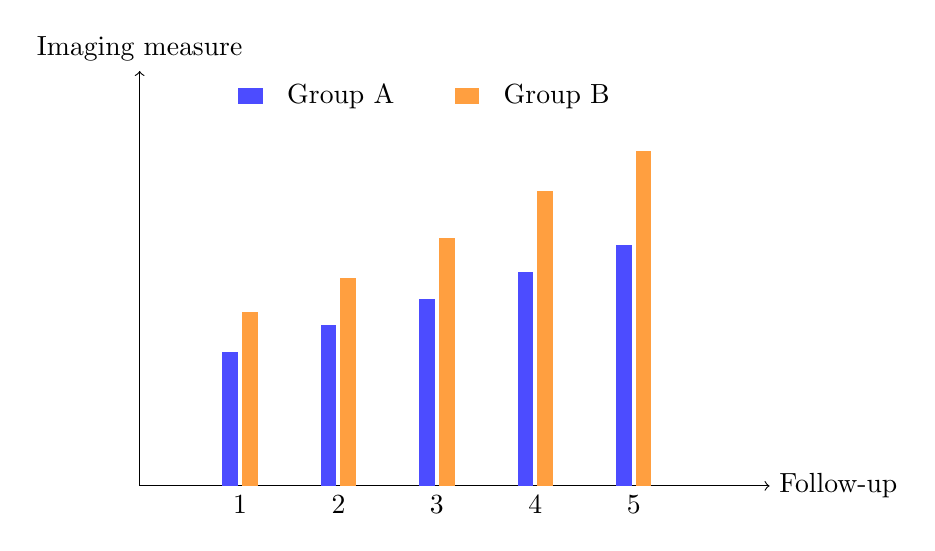
\begin{tikzpicture}[x=1.25cm,y=0.85cm]
    \draw[->] (0,0) -- (6.4,0) node[right] {Follow-up};
    \draw[->] (0,0) -- (0,6.2) node[above] {Imaging measure};
    \foreach \x/\a/\b in {1/2.0/2.6,2/2.4/3.1,3/2.8/3.7,4/3.2/4.4,5/3.6/5.0}
      {
        \fill[blue!70] (\x-0.16,0) rectangle (\x,{\a});
        \fill[orange!75] (\x+0.04,0) rectangle (\x+0.20,{\b});
      }
    \fill[blue!70] (1.0,5.7) rectangle (1.25,5.95);
    \node[anchor=west] at (1.4,5.82) {Group A};
    \fill[orange!75] (3.2,5.7) rectangle (3.45,5.95);
    \node[anchor=west] at (3.6,5.82) {Group B};
    \foreach \x in {1,...,5} \node[below] at (\x+0.02,0) {\x};
  \end{tikzpicture}
  \caption{Illustrative grouped measurements over five follow-up occasions}
  \label{fig:showcase-observations}
\end{figure}

When using an external image instead, place the image in a
\texttt{figures/} folder and replace the drawing code with
\verb|\includegraphics|, as shown in the README.

\section{Table, equation and quotation}

\subsection{Example table}

Table~\ref{tab:showcase-measures} has its number and title above the table.
The row and column headings include enough information for the example to be
understood independently of the surrounding paragraph.

\begin{table}[htbp]
  \caption{Illustrative measurements and reporting formats}
  \label{tab:showcase-measures}
  \centering
  \begin{tabular}{lll}
    \toprule
    Domain & Example measure & Reporting format \\
    \midrule
    Symptoms & Pain score & Mean (SD) \\
    Structure & Cartilage thickness & Millimetres \\
    Composition & T2 relaxation time & Milliseconds \\
    Function & Walking speed & Metres per second \\
    \bottomrule
  \end{tabular}
\end{table}

\subsection{Example equation}

Numbered equations can be referenced in the same way as figures and tables:
\begin{equation}
  \Delta Y = Y_{\mathrm{follow\text{-}up}} - Y_{\mathrm{baseline}}.
  \label{eq:showcase-change}
\end{equation}
Equation~\ref{eq:showcase-change} defines a simple change score. Short
mathematical expressions such as \(n=120\) can also appear within a sentence.

\subsection{Example quotation}

\begin{brightonquotation}
This indented passage demonstrates the single-spaced quotation environment.
Replace it with the quoted material, include a page number where appropriate
and provide the corresponding citation.
\end{brightonquotation}

\section{Footnote and endnote examples}

A footnote marker appears here.\footnote{This is a visible example footnote.
It is numbered automatically and printed at the bottom of the same page in
smaller, single-spaced text.} Footnotes should contain information needed to
understand the nearby text without interrupting the main sentence.

An endnote marker appears here.\endnote{This second example endnote was called
from the formatting-showcase chapter. It is collected with the earlier
endnote in the dedicated Endnotes section near the end of the thesis.}
The superscript marker beside the preceding sentence points to the numbered
entry printed in the separate \emph{Endnotes} section. It is not printed at
the bottom of this page. Endnotes are useful for additional material that can
be read separately from the immediate argument.

\section{Cross-references and chapter summary}

This chapter referred to Section~\ref{sec:showcase-headings},
Figure~\ref{fig:showcase-pathway}, Figure~\ref{fig:showcase-observations},
Table~\ref{tab:showcase-measures} and Equation~\ref{eq:showcase-change} without
typing their final numbers. The labels remain stable even if the content moves.

The source demonstrates running headings, multiple heading levels, ordinary
paragraphs, inline formatting, bullet points, numbered steps, description
lists, two figures, a table, an equation, a quotation, a footnote, an endnote
and cross-references. Delete the line
\verb|% !TeX root = ../main.tex
\chapter{Formatting Showcase}
\label{chap:formatting-showcase}

This chapter exists solely to make the template's features easy to inspect.
It can be deleted when beginning the real thesis. Every example is formatted
by \texttt{brightonthesis.sty}; the chapter file contains content and semantic
LaTeX commands, but no local margin, font or page-style settings.

The running header is visible above. It uses smaller type and shows the
candidate name, submission year and page number. It appears only in the
numbered main text. The formal page number is also retained at the bottom
centre. The option that enables the header is set near the top of
\texttt{main.tex}.

\section{Heading hierarchy}
\label{sec:showcase-headings}

Use headings to describe the structure of the argument. LaTeX calculates their
numbers, adds the required levels to the table of contents and updates
cross-references after compilation.

\subsection{A numbered subsection}
\label{sec:showcase-subsection}

This heading demonstrates the second level beneath a chapter. In a long thesis,
subsections help readers identify the distinct components of a method, result
or argument without making every short paragraph a separate section.

\subsubsection{A numbered subsubsection}
\label{sec:showcase-subsubsection}

This is the third displayed level beneath a chapter. The stylesheet gives it a
smaller, left-aligned heading while retaining automatic numbering. Use this
level sparingly so the hierarchy remains easy to follow.

\subsubsection{A second subsubsection}

The next heading number is generated automatically. If a section is moved to
another chapter, all its heading, figure, table and equation references update
after recompilation.

\subsection{Paragraphs and inline text}

Ordinary paragraphs are typed without formatting commands. A completely blank
line in the source begins a new paragraph. The stylesheet applies the approved
12-point font, one-and-a-half spacing, flush-left alignment and additional
space between paragraphs consistently across the thesis.

Use \emph{emphasis} for a term that needs modest emphasis and
\textbf{bold text} only where a strong visual distinction is genuinely useful.
File names and short pieces of code can be shown as
\texttt{chapters/06-formatting-showcase.tex}. A non-breaking space in a
reference, such as Figure~\ref{fig:showcase-pathway}, prevents the label and
number from being separated at a line ending.

\section{Lists}

Lists are useful when the items are genuinely parallel. They should not replace
connected explanatory prose simply to make the page look more varied.

\subsection{Bullet points}

The \texttt{itemize} environment creates bullet points:

\begin{itemize}
  \item define the population and sampling frame;
  \item describe acquisition and quality-control procedures;
  \item identify the primary and secondary outcomes;
  \item prespecify the statistical analysis; and
  \item report missing data and uncertainty.
\end{itemize}

Text following the list returns automatically to the ordinary paragraph style.
Punctuation is included here because the bullets form one continuing sentence.

\subsection{Numbered steps}

The \texttt{enumerate} environment is appropriate when order matters:

\begin{enumerate}
  \item Screen potential participants against the eligibility criteria.
  \item Obtain informed consent before research procedures begin.
  \item Acquire clinical and imaging measurements using the protocol.
  \item Perform quality control without reference to the later outcome.
  \item Conduct the prespecified analysis and report all relevant results.
\end{enumerate}

\subsection{Labelled descriptions}

A description list pairs a short label with explanatory text:

\begin{description}
  \item[Population] Adults with symptoms but without established radiographic
    osteoarthritis at baseline.
  \item[Exposure] A quantitative MRI measure obtained using a standardised
    acquisition and processing pipeline.
  \item[Outcome] Change in pain, function or structural status during follow-up.
\end{description}

\section{Figures and captions}

Figures are numbered by chapter, listed automatically in the list of figures
and referred to using labels. Captions appear below figures in accordance with
the Brighton guidance.

\subsection{Example figure one: process diagram}

Figure~\ref{fig:showcase-pathway} is a vector process diagram. Because it is
drawn in LaTeX, it remains sharp when enlarged in the PDF.

\begin{figure}[htbp]
  \centering
  \begin{tikzpicture}[
      node distance=1.1cm,
      every node/.style={font=\normalsize},
      box/.style={draw,rounded corners,minimum width=8.5cm,
        minimum height=1.05cm,align=center,fill=blue!8},
      arrow/.style={->,thick}
    ]
    \node[box] (question) {Research question and prespecified objectives};
    \node[box,below=of question] (measure) {Clinical and imaging measurements};
    \node[box,below=of measure] (analysis) {Quality control and statistical analysis};
    \node[box,below=of analysis] (interpret) {Interpretation and clinical relevance};
    \draw[arrow] (question) -- (measure);
    \draw[arrow] (measure) -- (analysis);
    \draw[arrow] (analysis) -- (interpret);
  \end{tikzpicture}
  \caption{Example pathway from research question to interpretation}
  \label{fig:showcase-pathway}
\end{figure}

\subsection{Example figure two: grouped observations}

Figure~\ref{fig:showcase-observations} demonstrates a second, visually distinct
figure and an automatically generated cross-reference.

\begin{figure}[htbp]
  \centering
  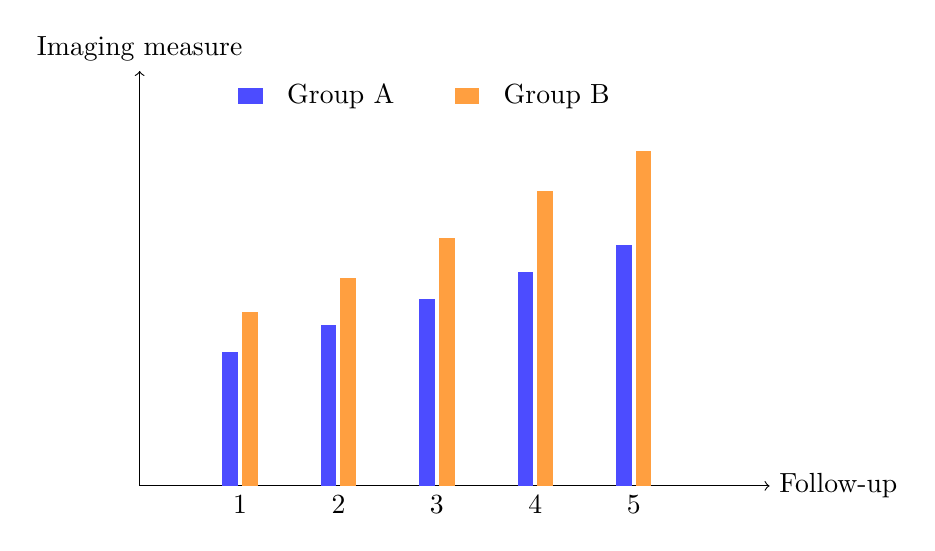
\begin{tikzpicture}[x=1.25cm,y=0.85cm]
    \draw[->] (0,0) -- (6.4,0) node[right] {Follow-up};
    \draw[->] (0,0) -- (0,6.2) node[above] {Imaging measure};
    \foreach \x/\a/\b in {1/2.0/2.6,2/2.4/3.1,3/2.8/3.7,4/3.2/4.4,5/3.6/5.0}
      {
        \fill[blue!70] (\x-0.16,0) rectangle (\x,{\a});
        \fill[orange!75] (\x+0.04,0) rectangle (\x+0.20,{\b});
      }
    \fill[blue!70] (1.0,5.7) rectangle (1.25,5.95);
    \node[anchor=west] at (1.4,5.82) {Group A};
    \fill[orange!75] (3.2,5.7) rectangle (3.45,5.95);
    \node[anchor=west] at (3.6,5.82) {Group B};
    \foreach \x in {1,...,5} \node[below] at (\x+0.02,0) {\x};
  \end{tikzpicture}
  \caption{Illustrative grouped measurements over five follow-up occasions}
  \label{fig:showcase-observations}
\end{figure}

When using an external image instead, place the image in a
\texttt{figures/} folder and replace the drawing code with
\verb|\includegraphics|, as shown in the README.

\section{Table, equation and quotation}

\subsection{Example table}

Table~\ref{tab:showcase-measures} has its number and title above the table.
The row and column headings include enough information for the example to be
understood independently of the surrounding paragraph.

\begin{table}[htbp]
  \caption{Illustrative measurements and reporting formats}
  \label{tab:showcase-measures}
  \centering
  \begin{tabular}{lll}
    \toprule
    Domain & Example measure & Reporting format \\
    \midrule
    Symptoms & Pain score & Mean (SD) \\
    Structure & Cartilage thickness & Millimetres \\
    Composition & T2 relaxation time & Milliseconds \\
    Function & Walking speed & Metres per second \\
    \bottomrule
  \end{tabular}
\end{table}

\subsection{Example equation}

Numbered equations can be referenced in the same way as figures and tables:
\begin{equation}
  \Delta Y = Y_{\mathrm{follow\text{-}up}} - Y_{\mathrm{baseline}}.
  \label{eq:showcase-change}
\end{equation}
Equation~\ref{eq:showcase-change} defines a simple change score. Short
mathematical expressions such as \(n=120\) can also appear within a sentence.

\subsection{Example quotation}

\begin{brightonquotation}
This indented passage demonstrates the single-spaced quotation environment.
Replace it with the quoted material, include a page number where appropriate
and provide the corresponding citation.
\end{brightonquotation}

\section{Footnote and endnote examples}

A footnote marker appears here.\footnote{This is a visible example footnote.
It is numbered automatically and printed at the bottom of the same page in
smaller, single-spaced text.} Footnotes should contain information needed to
understand the nearby text without interrupting the main sentence.

An endnote marker appears here.\endnote{This second example endnote was called
from the formatting-showcase chapter. It is collected with the earlier
endnote in the dedicated Endnotes section near the end of the thesis.}
The superscript marker beside the preceding sentence points to the numbered
entry printed in the separate \emph{Endnotes} section. It is not printed at
the bottom of this page. Endnotes are useful for additional material that can
be read separately from the immediate argument.

\section{Cross-references and chapter summary}

This chapter referred to Section~\ref{sec:showcase-headings},
Figure~\ref{fig:showcase-pathway}, Figure~\ref{fig:showcase-observations},
Table~\ref{tab:showcase-measures} and Equation~\ref{eq:showcase-change} without
typing their final numbers. The labels remain stable even if the content moves.

The source demonstrates running headings, multiple heading levels, ordinary
paragraphs, inline formatting, bullet points, numbered steps, description
lists, two figures, a table, an equation, a quotation, a footnote, an endnote
and cross-references. Delete the line
\verb|% !TeX root = ../main.tex
\chapter{Formatting Showcase}
\label{chap:formatting-showcase}

This chapter exists solely to make the template's features easy to inspect.
It can be deleted when beginning the real thesis. Every example is formatted
by \texttt{brightonthesis.sty}; the chapter file contains content and semantic
LaTeX commands, but no local margin, font or page-style settings.

The running header is visible above. It uses smaller type and shows the
candidate name, submission year and page number. It appears only in the
numbered main text. The formal page number is also retained at the bottom
centre. The option that enables the header is set near the top of
\texttt{main.tex}.

\section{Heading hierarchy}
\label{sec:showcase-headings}

Use headings to describe the structure of the argument. LaTeX calculates their
numbers, adds the required levels to the table of contents and updates
cross-references after compilation.

\subsection{A numbered subsection}
\label{sec:showcase-subsection}

This heading demonstrates the second level beneath a chapter. In a long thesis,
subsections help readers identify the distinct components of a method, result
or argument without making every short paragraph a separate section.

\subsubsection{A numbered subsubsection}
\label{sec:showcase-subsubsection}

This is the third displayed level beneath a chapter. The stylesheet gives it a
smaller, left-aligned heading while retaining automatic numbering. Use this
level sparingly so the hierarchy remains easy to follow.

\subsubsection{A second subsubsection}

The next heading number is generated automatically. If a section is moved to
another chapter, all its heading, figure, table and equation references update
after recompilation.

\subsection{Paragraphs and inline text}

Ordinary paragraphs are typed without formatting commands. A completely blank
line in the source begins a new paragraph. The stylesheet applies the approved
12-point font, one-and-a-half spacing, flush-left alignment and additional
space between paragraphs consistently across the thesis.

Use \emph{emphasis} for a term that needs modest emphasis and
\textbf{bold text} only where a strong visual distinction is genuinely useful.
File names and short pieces of code can be shown as
\texttt{chapters/06-formatting-showcase.tex}. A non-breaking space in a
reference, such as Figure~\ref{fig:showcase-pathway}, prevents the label and
number from being separated at a line ending.

\section{Lists}

Lists are useful when the items are genuinely parallel. They should not replace
connected explanatory prose simply to make the page look more varied.

\subsection{Bullet points}

The \texttt{itemize} environment creates bullet points:

\begin{itemize}
  \item define the population and sampling frame;
  \item describe acquisition and quality-control procedures;
  \item identify the primary and secondary outcomes;
  \item prespecify the statistical analysis; and
  \item report missing data and uncertainty.
\end{itemize}

Text following the list returns automatically to the ordinary paragraph style.
Punctuation is included here because the bullets form one continuing sentence.

\subsection{Numbered steps}

The \texttt{enumerate} environment is appropriate when order matters:

\begin{enumerate}
  \item Screen potential participants against the eligibility criteria.
  \item Obtain informed consent before research procedures begin.
  \item Acquire clinical and imaging measurements using the protocol.
  \item Perform quality control without reference to the later outcome.
  \item Conduct the prespecified analysis and report all relevant results.
\end{enumerate}

\subsection{Labelled descriptions}

A description list pairs a short label with explanatory text:

\begin{description}
  \item[Population] Adults with symptoms but without established radiographic
    osteoarthritis at baseline.
  \item[Exposure] A quantitative MRI measure obtained using a standardised
    acquisition and processing pipeline.
  \item[Outcome] Change in pain, function or structural status during follow-up.
\end{description}

\section{Figures and captions}

Figures are numbered by chapter, listed automatically in the list of figures
and referred to using labels. Captions appear below figures in accordance with
the Brighton guidance.

\subsection{Example figure one: process diagram}

Figure~\ref{fig:showcase-pathway} is a vector process diagram. Because it is
drawn in LaTeX, it remains sharp when enlarged in the PDF.

\begin{figure}[htbp]
  \centering
  \begin{tikzpicture}[
      node distance=1.1cm,
      every node/.style={font=\normalsize},
      box/.style={draw,rounded corners,minimum width=8.5cm,
        minimum height=1.05cm,align=center,fill=blue!8},
      arrow/.style={->,thick}
    ]
    \node[box] (question) {Research question and prespecified objectives};
    \node[box,below=of question] (measure) {Clinical and imaging measurements};
    \node[box,below=of measure] (analysis) {Quality control and statistical analysis};
    \node[box,below=of analysis] (interpret) {Interpretation and clinical relevance};
    \draw[arrow] (question) -- (measure);
    \draw[arrow] (measure) -- (analysis);
    \draw[arrow] (analysis) -- (interpret);
  \end{tikzpicture}
  \caption{Example pathway from research question to interpretation}
  \label{fig:showcase-pathway}
\end{figure}

\subsection{Example figure two: grouped observations}

Figure~\ref{fig:showcase-observations} demonstrates a second, visually distinct
figure and an automatically generated cross-reference.

\begin{figure}[htbp]
  \centering
  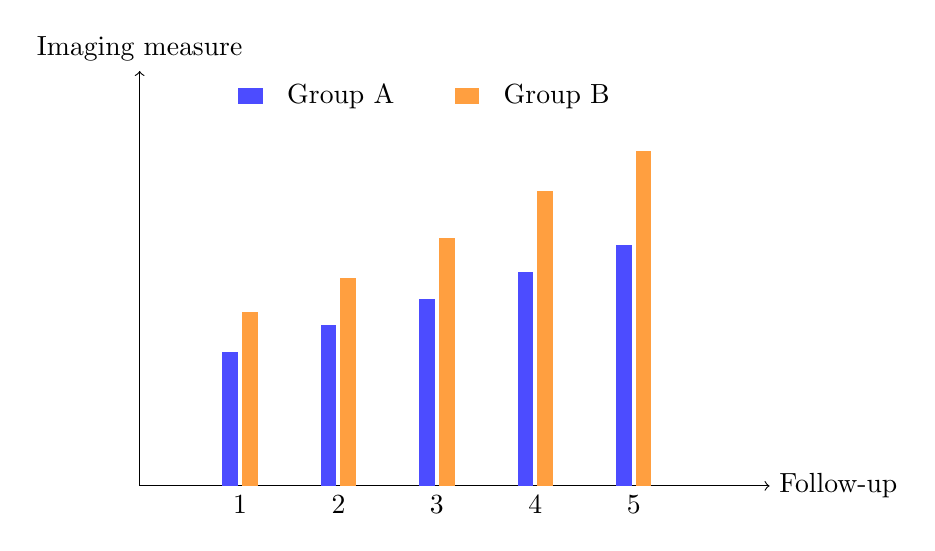
\begin{tikzpicture}[x=1.25cm,y=0.85cm]
    \draw[->] (0,0) -- (6.4,0) node[right] {Follow-up};
    \draw[->] (0,0) -- (0,6.2) node[above] {Imaging measure};
    \foreach \x/\a/\b in {1/2.0/2.6,2/2.4/3.1,3/2.8/3.7,4/3.2/4.4,5/3.6/5.0}
      {
        \fill[blue!70] (\x-0.16,0) rectangle (\x,{\a});
        \fill[orange!75] (\x+0.04,0) rectangle (\x+0.20,{\b});
      }
    \fill[blue!70] (1.0,5.7) rectangle (1.25,5.95);
    \node[anchor=west] at (1.4,5.82) {Group A};
    \fill[orange!75] (3.2,5.7) rectangle (3.45,5.95);
    \node[anchor=west] at (3.6,5.82) {Group B};
    \foreach \x in {1,...,5} \node[below] at (\x+0.02,0) {\x};
  \end{tikzpicture}
  \caption{Illustrative grouped measurements over five follow-up occasions}
  \label{fig:showcase-observations}
\end{figure}

When using an external image instead, place the image in a
\texttt{figures/} folder and replace the drawing code with
\verb|\includegraphics|, as shown in the README.

\section{Table, equation and quotation}

\subsection{Example table}

Table~\ref{tab:showcase-measures} has its number and title above the table.
The row and column headings include enough information for the example to be
understood independently of the surrounding paragraph.

\begin{table}[htbp]
  \caption{Illustrative measurements and reporting formats}
  \label{tab:showcase-measures}
  \centering
  \begin{tabular}{lll}
    \toprule
    Domain & Example measure & Reporting format \\
    \midrule
    Symptoms & Pain score & Mean (SD) \\
    Structure & Cartilage thickness & Millimetres \\
    Composition & T2 relaxation time & Milliseconds \\
    Function & Walking speed & Metres per second \\
    \bottomrule
  \end{tabular}
\end{table}

\subsection{Example equation}

Numbered equations can be referenced in the same way as figures and tables:
\begin{equation}
  \Delta Y = Y_{\mathrm{follow\text{-}up}} - Y_{\mathrm{baseline}}.
  \label{eq:showcase-change}
\end{equation}
Equation~\ref{eq:showcase-change} defines a simple change score. Short
mathematical expressions such as \(n=120\) can also appear within a sentence.

\subsection{Example quotation}

\begin{brightonquotation}
This indented passage demonstrates the single-spaced quotation environment.
Replace it with the quoted material, include a page number where appropriate
and provide the corresponding citation.
\end{brightonquotation}

\section{Footnote and endnote examples}

A footnote marker appears here.\footnote{This is a visible example footnote.
It is numbered automatically and printed at the bottom of the same page in
smaller, single-spaced text.} Footnotes should contain information needed to
understand the nearby text without interrupting the main sentence.

An endnote marker appears here.\endnote{This second example endnote was called
from the formatting-showcase chapter. It is collected with the earlier
endnote in the dedicated Endnotes section near the end of the thesis.}
The superscript marker beside the preceding sentence points to the numbered
entry printed in the separate \emph{Endnotes} section. It is not printed at
the bottom of this page. Endnotes are useful for additional material that can
be read separately from the immediate argument.

\section{Cross-references and chapter summary}

This chapter referred to Section~\ref{sec:showcase-headings},
Figure~\ref{fig:showcase-pathway}, Figure~\ref{fig:showcase-observations},
Table~\ref{tab:showcase-measures} and Equation~\ref{eq:showcase-change} without
typing their final numbers. The labels remain stable even if the content moves.

The source demonstrates running headings, multiple heading levels, ordinary
paragraphs, inline formatting, bullet points, numbered steps, description
lists, two figures, a table, an equation, a quotation, a footnote, an endnote
and cross-references. Delete the line
\verb|% !TeX root = ../main.tex
\chapter{Formatting Showcase}
\label{chap:formatting-showcase}

This chapter exists solely to make the template's features easy to inspect.
It can be deleted when beginning the real thesis. Every example is formatted
by \texttt{brightonthesis.sty}; the chapter file contains content and semantic
LaTeX commands, but no local margin, font or page-style settings.

The running header is visible above. It uses smaller type and shows the
candidate name, submission year and page number. It appears only in the
numbered main text. The formal page number is also retained at the bottom
centre. The option that enables the header is set near the top of
\texttt{main.tex}.

\section{Heading hierarchy}
\label{sec:showcase-headings}

Use headings to describe the structure of the argument. LaTeX calculates their
numbers, adds the required levels to the table of contents and updates
cross-references after compilation.

\subsection{A numbered subsection}
\label{sec:showcase-subsection}

This heading demonstrates the second level beneath a chapter. In a long thesis,
subsections help readers identify the distinct components of a method, result
or argument without making every short paragraph a separate section.

\subsubsection{A numbered subsubsection}
\label{sec:showcase-subsubsection}

This is the third displayed level beneath a chapter. The stylesheet gives it a
smaller, left-aligned heading while retaining automatic numbering. Use this
level sparingly so the hierarchy remains easy to follow.

\subsubsection{A second subsubsection}

The next heading number is generated automatically. If a section is moved to
another chapter, all its heading, figure, table and equation references update
after recompilation.

\subsection{Paragraphs and inline text}

Ordinary paragraphs are typed without formatting commands. A completely blank
line in the source begins a new paragraph. The stylesheet applies the approved
12-point font, one-and-a-half spacing, flush-left alignment and additional
space between paragraphs consistently across the thesis.

Use \emph{emphasis} for a term that needs modest emphasis and
\textbf{bold text} only where a strong visual distinction is genuinely useful.
File names and short pieces of code can be shown as
\texttt{chapters/06-formatting-showcase.tex}. A non-breaking space in a
reference, such as Figure~\ref{fig:showcase-pathway}, prevents the label and
number from being separated at a line ending.

\section{Lists}

Lists are useful when the items are genuinely parallel. They should not replace
connected explanatory prose simply to make the page look more varied.

\subsection{Bullet points}

The \texttt{itemize} environment creates bullet points:

\begin{itemize}
  \item define the population and sampling frame;
  \item describe acquisition and quality-control procedures;
  \item identify the primary and secondary outcomes;
  \item prespecify the statistical analysis; and
  \item report missing data and uncertainty.
\end{itemize}

Text following the list returns automatically to the ordinary paragraph style.
Punctuation is included here because the bullets form one continuing sentence.

\subsection{Numbered steps}

The \texttt{enumerate} environment is appropriate when order matters:

\begin{enumerate}
  \item Screen potential participants against the eligibility criteria.
  \item Obtain informed consent before research procedures begin.
  \item Acquire clinical and imaging measurements using the protocol.
  \item Perform quality control without reference to the later outcome.
  \item Conduct the prespecified analysis and report all relevant results.
\end{enumerate}

\subsection{Labelled descriptions}

A description list pairs a short label with explanatory text:

\begin{description}
  \item[Population] Adults with symptoms but without established radiographic
    osteoarthritis at baseline.
  \item[Exposure] A quantitative MRI measure obtained using a standardised
    acquisition and processing pipeline.
  \item[Outcome] Change in pain, function or structural status during follow-up.
\end{description}

\section{Figures and captions}

Figures are numbered by chapter, listed automatically in the list of figures
and referred to using labels. Captions appear below figures in accordance with
the Brighton guidance.

\subsection{Example figure one: process diagram}

Figure~\ref{fig:showcase-pathway} is a vector process diagram. Because it is
drawn in LaTeX, it remains sharp when enlarged in the PDF.

\begin{figure}[htbp]
  \centering
  \begin{tikzpicture}[
      node distance=1.1cm,
      every node/.style={font=\normalsize},
      box/.style={draw,rounded corners,minimum width=8.5cm,
        minimum height=1.05cm,align=center,fill=blue!8},
      arrow/.style={->,thick}
    ]
    \node[box] (question) {Research question and prespecified objectives};
    \node[box,below=of question] (measure) {Clinical and imaging measurements};
    \node[box,below=of measure] (analysis) {Quality control and statistical analysis};
    \node[box,below=of analysis] (interpret) {Interpretation and clinical relevance};
    \draw[arrow] (question) -- (measure);
    \draw[arrow] (measure) -- (analysis);
    \draw[arrow] (analysis) -- (interpret);
  \end{tikzpicture}
  \caption{Example pathway from research question to interpretation}
  \label{fig:showcase-pathway}
\end{figure}

\subsection{Example figure two: grouped observations}

Figure~\ref{fig:showcase-observations} demonstrates a second, visually distinct
figure and an automatically generated cross-reference.

\begin{figure}[htbp]
  \centering
  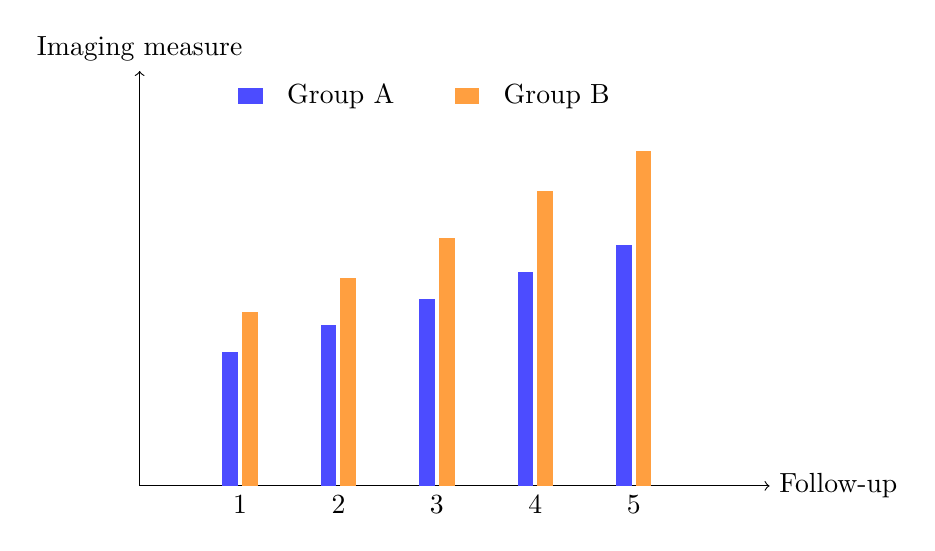
\begin{tikzpicture}[x=1.25cm,y=0.85cm]
    \draw[->] (0,0) -- (6.4,0) node[right] {Follow-up};
    \draw[->] (0,0) -- (0,6.2) node[above] {Imaging measure};
    \foreach \x/\a/\b in {1/2.0/2.6,2/2.4/3.1,3/2.8/3.7,4/3.2/4.4,5/3.6/5.0}
      {
        \fill[blue!70] (\x-0.16,0) rectangle (\x,{\a});
        \fill[orange!75] (\x+0.04,0) rectangle (\x+0.20,{\b});
      }
    \fill[blue!70] (1.0,5.7) rectangle (1.25,5.95);
    \node[anchor=west] at (1.4,5.82) {Group A};
    \fill[orange!75] (3.2,5.7) rectangle (3.45,5.95);
    \node[anchor=west] at (3.6,5.82) {Group B};
    \foreach \x in {1,...,5} \node[below] at (\x+0.02,0) {\x};
  \end{tikzpicture}
  \caption{Illustrative grouped measurements over five follow-up occasions}
  \label{fig:showcase-observations}
\end{figure}

When using an external image instead, place the image in a
\texttt{figures/} folder and replace the drawing code with
\verb|\includegraphics|, as shown in the README.

\section{Table, equation and quotation}

\subsection{Example table}

Table~\ref{tab:showcase-measures} has its number and title above the table.
The row and column headings include enough information for the example to be
understood independently of the surrounding paragraph.

\begin{table}[htbp]
  \caption{Illustrative measurements and reporting formats}
  \label{tab:showcase-measures}
  \centering
  \begin{tabular}{lll}
    \toprule
    Domain & Example measure & Reporting format \\
    \midrule
    Symptoms & Pain score & Mean (SD) \\
    Structure & Cartilage thickness & Millimetres \\
    Composition & T2 relaxation time & Milliseconds \\
    Function & Walking speed & Metres per second \\
    \bottomrule
  \end{tabular}
\end{table}

\subsection{Example equation}

Numbered equations can be referenced in the same way as figures and tables:
\begin{equation}
  \Delta Y = Y_{\mathrm{follow\text{-}up}} - Y_{\mathrm{baseline}}.
  \label{eq:showcase-change}
\end{equation}
Equation~\ref{eq:showcase-change} defines a simple change score. Short
mathematical expressions such as \(n=120\) can also appear within a sentence.

\subsection{Example quotation}

\begin{brightonquotation}
This indented passage demonstrates the single-spaced quotation environment.
Replace it with the quoted material, include a page number where appropriate
and provide the corresponding citation.
\end{brightonquotation}

\section{Footnote and endnote examples}

A footnote marker appears here.\footnote{This is a visible example footnote.
It is numbered automatically and printed at the bottom of the same page in
smaller, single-spaced text.} Footnotes should contain information needed to
understand the nearby text without interrupting the main sentence.

An endnote marker appears here.\endnote{This second example endnote was called
from the formatting-showcase chapter. It is collected with the earlier
endnote in the dedicated Endnotes section near the end of the thesis.}
The superscript marker beside the preceding sentence points to the numbered
entry printed in the separate \emph{Endnotes} section. It is not printed at
the bottom of this page. Endnotes are useful for additional material that can
be read separately from the immediate argument.

\section{Cross-references and chapter summary}

This chapter referred to Section~\ref{sec:showcase-headings},
Figure~\ref{fig:showcase-pathway}, Figure~\ref{fig:showcase-observations},
Table~\ref{tab:showcase-measures} and Equation~\ref{eq:showcase-change} without
typing their final numbers. The labels remain stable even if the content moves.

The source demonstrates running headings, multiple heading levels, ordinary
paragraphs, inline formatting, bullet points, numbered steps, description
lists, two figures, a table, an equation, a quotation, a footnote, an endnote
and cross-references. Delete the line
\verb|\include{chapters/06-formatting-showcase}| from \texttt{main.tex} when
this demonstration is no longer required.
| from \texttt{main.tex} when
this demonstration is no longer required.
| from \texttt{main.tex} when
this demonstration is no longer required.
| from \texttt{main.tex} when
this demonstration is no longer required.
